\documentclass[class=book, crop=false, oneside, 12pt]{standalone}
\usepackage{standalone}
\usepackage{amsmath}
\usepackage{../../style}
\graphicspath{{./assets/images/}}

% arara: pdflatex: { synctex: yes, shell: yes }
% arara: latexmk: { clean: partial }
\begin{document}

\chapter{Corrente elettrica}

\section{Conduzione elettrica}

I materiali conduttori solidi sono costituiti da un reticolo spaziale ai cui vertici si trovano gli ioni positivi (atomi che hanno perso uno o più elettroni) e al cui interno si muovono gli elettroni liberi. 
In un metallo questi sono gli unici portatori mobili di carica. 
Nel rame e nell'argento, in cui c'è un elettrone libero per atomo, il numero di elettroni per unità di volume coincide con il numero di atomi per unità di volume e abbiamo rispettivamente
\begin{equation*}
    n = \frac{N_A \rho}{A} = \frac{6.022 \cdot 10^{26} \cdot 8.96 \cdot 10^3}{63.55} = 8.49 \cdot 10^{28} \text{ elettroni / }m^3
\end{equation*}
\begin{equation*}
    n = \frac{6.022 \cdot 10^{26} \cdot 10.5 \cdot 10^3}{107.87} = 5.86 \cdot 10^{28} \text{ elettroni / }m^3
\end{equation*}

In qualsiasi volume \(\tau\), piccolo su scala macroscopica, ma contenente un numero \(N\) di elettroni abbastanza elevato, la velocità media è nulla: 
\begin{equation*}
    \overrightarrow{v}_m = \frac{1}{N} \sum_i \overrightarrow{v}_i = 0
\end{equation*}
indicando con \(\overrightarrow{v}_i\) le velocità dei singoli elettroni. 
Ciò vuol dire che non esiste una direzione di moto preferenziale per gli elettroni.

Se si mettono a contatto due conduttori \(C_1\) e \(C_2\) isolati, a potenziali \(V_1\) e \(V_2\) diversi, si raggiunge una condizione di equilibrio in cui entrambi i conduttori si portano allo stesso potenziale \(V\). 
Nel processo un certo numero di elettroni passa dal conduttore a potenziale minore a quello a potenziale maggiore, sotto l'azione del campo elettrico \(\overrightarrow{E}\) dovuto alla differenza di potenziale, \(\Delta V\). 
Questo moto ordinato di elettroni in una certa direzione costituisce una \emph{corrente elettrica} e il fenomeno è un esempio di \emph{conduzione elettrica}.

La corrente elettrica in questo caso specifico dura soltanto un tempo molto breve che impedisce l'esecuzione di studi sistematici del fenomeno. 

A tale scopo è necessario un dispositivo capace di mantenere una differenza di potenziale, e quindi un campo elettrico, tra due conduttori a contatto ovvero tra due punti di uno stesso conduttore. 
Così facendo il flusso di elettroni può durare per molto tempo e quindi nel conduttore si instaura una corrente elettrica stabile, in un regime di equilibrio dinamico e non più di equilibrio elettrostatico.

Un qualsiasi dispositivo con le caratteristiche appena descritte è definito come \emph{generatore di forza elettromotrice (f.e.m.)}.

\section{Corrente elettrica}

Supponiamo che in una certa regione di un conduttore ci siano \(n\) portatori di carica \(+e\) per unità di volume e che in essa agisca un campo elettrico \(\overrightarrow{E}\) prodotto da un generatore di forza elettromotrice; i portatori si muovono sotto l'azione della forza elettrica \(\overrightarrow{F} = e \overrightarrow{E}\), acquistando, la velocità \(v_d\) lungo la direzione del campo elettrico \(\overrightarrow{E}\), detta velocità di deriva. 
Tale moto dà origine ad una corrente elettrica.

Consideriamo una superficie \(\Sigma\) tracciata all'interno del conduttore: detta \(\Delta q\) la carica che passa nel tempo \(\Delta t\) attraverso la superficie si definisce intensità di corrente media la grandezza:
\begin{equation*}
    i_m = \frac{\Delta q}{\Delta t}
\end{equation*}

La intensità di corrente istantanea è definita come il limite per \(\Delta t \rightarrow 0\) della intensità media:
\begin{equation*}
    i = \lim_{\Delta t \rightarrow 0 } \frac{\Delta q}{\Delta t} = \frac{dq}{dt}
\end{equation*} 

\begin{figure}[h]
    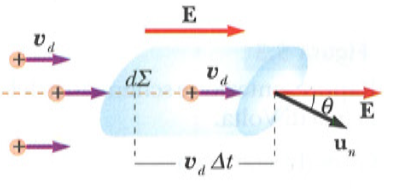
\includegraphics[scale=0.6]{intensita_corrente_superficie.png}
    \centering
    \caption{}
\end{figure}

Per mettere in relazione la corrente elettrica con il moto delle cariche ci riferiamo a una superficie infinitesima \(d\Sigma\): la cui normale \(\overrightarrow{u}_n\) formi un angolo e con il campo elettrico \(\overrightarrow{E}\) e quindi con la velocità \(\overrightarrow{v}_d\) delle cariche positive. 
Nel tempo \(\Delta t\) le cariche percorrono la distanza \(v_d \Delta t\) per cui la carica complessiva che passa attraverso \(d\Sigma\): nel tempo \(\Delta t\) è quella contenuta nel volume infinitesimo \(d \tau\) definito da \(d \Sigma\): e \(v_d \Delta t\):
\begin{equation*}
    \Delta \tau = v_d \Delta t d \Sigma \cos \theta \ , \ \Delta q = n_{+} e d \tau = n_{+} e v_d d \Sigma \cos \theta \Delta t
\end{equation*}

La carica che passa nell'unità di tempo attraverso \(d \Sigma\):, cioè l'intensità di corrente attraverso \(d \Sigma\):
\begin{equation*}
    di = n_{+} e v_d d \Sigma \cos \theta
\end{equation*}

Definiamo la densità di corrente \(j\) come
\begin{equation}
    \overrightarrow{j} = n_{+} e \overrightarrow{v}_d
\end{equation}
e riscriviamo 
\begin{equation} \label{intensita_infinitesima}
    di = \overrightarrow{j} \cdot \overrightarrow{u}_n d \Sigma
\end{equation}

L'intensità di corrente attraverso la superficie finita \(\Sigma\): si ottiene integrando (\ref{intensita_infinitesima})
\begin{equation} \label{intensita_di_corrente}
    i = \int_{\Sigma} \overrightarrow{j} \cdot \overrightarrow{u}_n d \Sigma
\end{equation}
essa \emph{risulta eguale al flusso del vettore densità di corrente attraverso la superficie} \(\Sigma\).

In particolare se la superficie \(\Sigma\): è ortogonale a \(\overrightarrow{j}\), cioè a \(\overrightarrow{v}_d\) e \(\overrightarrow{j}\) ha lo stesso valore in tutti i punti di \(\Sigma\),
\begin{equation}
    i = j \Sigma \ , \ j = \frac{i}{\Sigma}
\end{equation}
\emph{la densità di corrente è la corrente che attraversa l'unità di superficie perpendicolare alla direzione del moto delle cariche ( e resta così giustificato il nome densità di corrente). }

Se, come nei conduttori metallici, i portatori di carica sono negativi, fissata la direzione e il verso di \(\overrightarrow{E}\) la velocità di deriva \(\overrightarrow{v}_{-}\) è diretta in verso opposto rispetto al campo elettrico. 
Il vettore \(-e v_{-}\) ha invece lo stesso verso di \(\overrightarrow{E}\) e la densità di corrente, detto \(v_{-}\) il numero di portatori per unità di volume, è
\begin{equation}
    \overrightarrow{j} = -n_{-} e \overrightarrow{v}_{-}
\end{equation}
\emph{parallela e concorde } al campo elettrico.

Che la densità di corrente sia sempre concorde a \(\overrightarrow{E}\), discende dalla definizione di \(\overrightarrow{j}\) come prodotto della carica per unità di volume ( con il suo segno) per la velocità di deriva e riflette la circostanza sperimentale che su scala macroscopica non è possibile correlare il verso della corrente al segno dei portatori di carica: fissata una data differenza di potenziale gli stessi effetti si hanno se la conduzione è dovuta a cariche positive con moto concorde a \(\overrightarrow{E}\) oppure a cariche negative con moto discorde a \(\overrightarrow{E}\). 

In base a queste considerazioni si assume convenzionalmente come verso della corrente quello del moto delle cariche positive, ovvero quello che va dai punti a potenziale maggiore ai punti a potenziale minore.

\subsection{Corrente elettrica stazionaria}

\begin{figure}[h]
    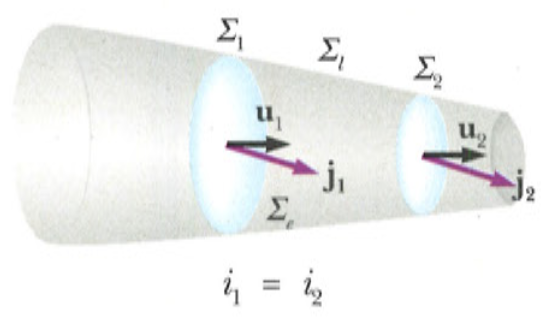
\includegraphics[scale=0.6]{corrente_elettrica_stazionaria.png}
    \centering
    \caption{}
\end{figure}

Consideriamo un conduttore percorso da una corrente di densità \(\overrightarrow{j}\). 
Se \(\Sigma_1\) e \(\Sigma_2\) sono due diverse sezioni del conduttore, le intensità di corrente attraverso le due sezioni sono, in base alla (\ref{intensita_di_corrente}),
\begin{equation*}
    i_1 = \int_{\Sigma_1} \overrightarrow{j}_1 \cdot \overrightarrow{u}_1 d \Sigma_1 \ , \ i_2 = \int_{\Sigma_2} \overrightarrow{j}_2 \cdot \overrightarrow{u}_2 d \Sigma_2
\end{equation*}
e rappresentano rispettivamente la carica che \emph{entra} e la carica che \emph{esce} nell'unità di tempo nel volume delimitato da \(\Sigma_1, \Sigma_2\) e dalla superficie laterale \(\Sigma_1\) attraverso la quale non c'è flusso di carica. 
Se si fa l'ipotesi che nell'interno del tronco di cono di basi \(\Sigma_1, \Sigma_2\) non vari nel tempo la carica, allora: 
\begin{equation}
    i_1 = i_2
\end{equation}
Questa condizione è detta di stazionarietà: \emph{in condizioni stazionarie l'intensità di corrente è costante attraverso ogni sezione del conduttore}. 

\section{Legge di Ohm della conduzione elettrica}

In un conduttore sottoposto ad una differenza di potenziale si stabilisce, in regime stazionario, che la densità di corrente \(\overrightarrow{j}\) legata al campo elettrico \(\overrightarrow{E}\) dalla relazione: 
\begin{equation} \label{legge_di_ohm_1}
    \overrightarrow{j} = \sigma \overrightarrow{E}
\end{equation}
con \(\overrightarrow{\sigma}\) una grandezza caratteristica del conduttore, detta \emph{conduttività elettrica}. 

La legge (\ref{legge_di_ohm_1}), nota come legge di Ohm della conduttività elettrica, venne stabilita sperimentalmente e fu verificata anche nella conduzione nei gas e nei liquidi, in cui siano presenti portatori di carica liberi. 
Essa definisce, all'interno di un conduttore percorso da corrente, il campo vettoriale \(\overrightarrow{j}\), le cui linee sono parallele e concordi alle linee del campo vettoriale \(\overrightarrow{E}\) che dà origine alla corrente. 

La legge di Ohm molto spesso è scritta nella forma:
\begin{equation}
    \overrightarrow{E} = \rho \overrightarrow{j}
\end{equation} 
dove la grandezza
\begin{equation}
    \overrightarrow{\rho} = \frac{1}{\sigma}
\end{equation}
È chiamata resistività del conduttore. 
Minore è la resistività del conduttore, maggiore è la densità di corrente che può circolare in un conduttore a parità di campo elettrico \(E\).

Applichiamo la legge di Ohm ad un conduttore metallico cilindrico di lunghezza \(h\) e sezione \(\Sigma\). 
Ai capi del conduttore è applicata, tramite un generatore di forza elettromotrice, una differenza di potenziale \(V = V_A - V_B\).
Il regime è stazionario, l'intensità di corrente ha lo stesso valore attraverso qualsiasi sezione del conduttore ed è legata al campo elettrico, in base a (5.5), dalla
\begin{equation*}
    E = \rho j = \frac{\rho}{\Sigma} i
\end{equation*}
Tra campo elettrico e differenza di potenziale sussiste la relazione 
\begin{equation*} 
    V = V_A - V_B = \int_A^B \overrightarrow{E} \cdot d \overrightarrow{s} = E h
\end{equation*}
e in definitiva 
\begin{equation}
    V = \frac{\rho h}{\Sigma} i
\end{equation} \label{differenza_di_potenziale_2}
Chiamando \emph{resistenza del conduttore} in esame la grandezza
\begin{equation}
    R = \rho \frac{h}{\Sigma}
\end{equation}
la (\ref{differenza_di_potenziale_2}) diviene
\begin{equation} \label{legge_di_ohm_2}
    V = R i
\end{equation}
nota come \emph{legge di Ohm per i conduttori metallici}.

Se la sezione del conduttore è variabile, per un tratto lungo \(dh\) e di sezione \(\Sigma\) scriviamo 
\begin{equation*}
    -d V = \overrightarrow{E} \cdot d \overrightarrow{s} = \rho \frac{dh}{\Sigma} i 
\end{equation*}
e integrando lungo tutto il conduttore otteniamo di nuovo:
\begin{equation*}
    V = V_A - V_B = \int_A^B \overrightarrow{E} \cdot d \overrightarrow{s} = R i
\end{equation*}
se indichiamo come \emph{resistenza del conduttore} la grandezza
\begin{equation}
    R = \int_A^B \rho \frac{dh }{\Sigma}
\end{equation}
e ricordiamo che l'intensità di corrente è la stessa in ogni sezione. 

Pertanto in regime stazionario il rapporto tra la differenza di potenziale applicata ai capi di un conduttore metallico e l'intensità di corrente che a seguito di ciò l'attraversa è pari a una grandezza, detta resistenza del conduttore, che dipende solamente dalla natura del conduttore (resistività \(\rho\)) e dalle sue dimensioni.

\subsection{Potenza, effetto Joule}

Consideriamo una carica \(dq\) che si muova attraversando la differenza di potenziale \(V= V_A -V_B\), per questo spostamento viene compiuto dal campo elettrico agente il lavoro:
\begin{equation*}
    d W = V dq = V i dt
\end{equation*}
e spera pertanto la \emph{potenza elettrica}
\begin{equation}
    \mathcal{P} = \frac{dW}{dt} = V i
\end{equation}

Se vale la legge di Ohm (\ref{legge_di_ohm_2})
\begin{equation}
    \mathcal{P} = R i^2 = \frac{V^2}{R}
\end{equation}

Il passaggio di corrente attraverso un conduttore metallico per un tempo \(t\) comporta dunque il \emph{lavoro} 
\begin{equation}
    W = \int_0^t \mathcal{P} dt = \int_0^t R i^2 dt
\end{equation}
che, se la corrente è costante nel tempo, si riduce a
\begin{equation}
    W = R i^2 t
\end{equation}
Questo lavoro è necessario per vincere la resistenza opposta dal reticolo cristallino al moto ordinato degli elettroni e, da un punto di vista termodinamico, esso viene assorbito dal conduttore la cui energia interna aumenta. 
Di conseguenza aumenta la temperatura del conduttore: se esso è isolato termicamente dall'ambiente il processo porta alla fusione del metallo; se invece il conduttore è in contatto termico con l'ambiente la sua temperatura cresce fino a che si raggiunge uno stato di equilibrio in cui l'energia interna non varia più e il lavoro elettrico viene ceduto all'ambiente sotto forma di calore (purché naturalmente la temperatura di equilibrio sia inferiore alla temperatura di fusione del conduttore). 

L'effetto di riscaldamento di un conduttore percorso da corrente si chiama \emph{effetto Joule}. 

\section{Resistori in serie e in parallelo}

Conduttori ohmici caratterizzati da un determinato valore della resistenza (alla temperatura ambiente) sono elementi molto usati nei circuiti elettrici. 
Essi vengono chiamati resistori e oltre al valore della resistenza viene sempre precisato il valore massimo della potenza che può essere in essi dissipata senza causare alterazioni irreversibili.

\subsection{Resistori in serie}

Due resistori sono collegati in serie, quando hanno un estremo in comune: in regime stazionario l'\emph{intensità di corrente che li attraversa è la stessa}. 
Applichiamo a ciascun resistore la legge di Ohm e sommiamo:
\begin{equation*}
    V_A - V_B = R_1 i \ , \ V_B - V_C = R_2 i 
\end{equation*}
\begin{equation*}
    V_A - V_C = \left(R_1 + R_2 \right) i = R_{eq} i
\end{equation*}

I due resistori in serie presentano la \emph{resistenza equivalente}:
\begin{equation*}
    R_{eq} = R_1 + R_2
\end{equation*}
Tale relazione si generalizza subito a un qualsiasi numero di resistori in serie
\begin{equation}
    R_{eq} = R_1 + R_2 + ... R_n
\end{equation}
\emph{in un collegamento in serie ciascun resistore è attraversato dalla stessa corrente; la resistenza equivalente è somma della resistenza dei singoli componenti}.

\subsection{Resistori in parallelo}

Due resistori si dicono in parallelo quando sono collegati tra loro in entrambi gli estremi. 
In questo caso l'elemento comune ai due resistori è la differenza di potenziale \(V = V_A -V_B\) e quindi, in base alla legge di Ohm, essi sono attraversati da due correnti \(i_1, i_2\), diverse se sono diversi i valori delle resistenze \(R_1\) e \(R_2\).

I due resistori in parallelo presentano la resistenza equivalente: 
\begin{equation*}
    \frac{1}{R_{eq}} = \frac{1}{R_1} + \frac{1}{R_2}
\end{equation*}
Anche questa relazione si estende ad un numero qualsiasi di resistori collegati in parallelo: 
\begin{equation}
    \frac{1}{R_{eq}} = \frac{1}{R_1} + \frac{1}{R_2} + ... + \frac{1}{R_n}
\end{equation}
\emph{in un collegamento in parallelo la differenza di potenziale è la stessa ai capi di ciascun resistore; l'inverso della resistenza equivalente è uguale alla somma degli inversi di ciascun componente}.

In un collegamento in parallelo la resistenza equivalente è minore del valore di ciascun componente.  
Attraverso combinazioni di serie e parallelo si può in pratica realizzare qualsiasi valore di resistenza.

\section{Forza elettromotrice}

Tale relazione applicata a un circuito chiuso diventa
\begin{equation} \label{fem}
    \oint \overrightarrow{E} \cdot d \overrightarrow{s} = R_T i 
\end{equation}
essendo \(R_T\) resistenza totale del circuito stesso.

\begin{figure}[h]
    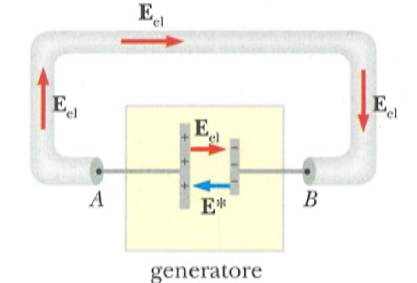
\includegraphics[scale=0.6]{campi_circuito.png}
    \centering
    \caption{}
\end{figure}

Il primo membro di (\ref{fem}) coincide con la definizione di forza elettromotrice \((f.e.m.)\) e pertanto la (\ref{fem}) afferma che per ottenere nel circuito una corrente di intensità i è necessaria la presenza nel circuito di una sorgente di f.e.m. ovvero di un campo \(\overrightarrow{E}\) la cui circuitazione non sia nulla. 
Ne segue che non può essere un campo elettrostatico \(E_{el}\) a fare circolare le cariche nel circuito in quanto esso è conservativo e la corrispondente forza elettromotrice è sempre nulla. 
La sorgente di forza elettromotrice deve invece avere al suo interno forze di natura non elettrostatica, \emph{non conservative}, che possono determinare il moto continuo delle cariche. 

Il campo elettrostatico \(\overrightarrow{E_{el}}\) prodotto da tali cariche è sempre diretto da \(\) verso \(B\), sia nel conduttore che all'interno del generatore e pertanto la sua forza elettromotrice è nulla. 
Per fare circolare corrente ci deve essere all'interno del generatore un campo \( E*\) di natura non elettrostatica, che chiamiamo campo elettromotore, capace di far muovere le cariche all'interno del generatore contro il campo elettrostatico \(E_{el}\).
L'integrale di \(E*\) lungo il circuito è: 
\begin{equation}
    \mathcal{E} = \oint \overrightarrow{E*} \cdot d \overrightarrow{l} = \int_A^B \overrightarrow{E*} \cdot d \overrightarrow{l}
\end{equation}
pari alla tensione dello stesso tra \(A\) e \(B\), calcolata lungo una linea interna al generatore.

Il dispositivo che genera il campo elettromotore, e quindi la forza elettromotrice, può sfruttare azioni meccaniche, reazioni chimiche (pile e accumulatori), il fenomeno dell'induzione elettromagnetica.

In ogni caso il generatore è caratterizzato oltre che dalla forza elettromotrice dalla sua resistenza interna \(r\), per la quale vale la legge di Ohm quando è percorsa dalla corrente \(i\).
\begin{equation*}
    V_B + \mathcal{E} - ri - Ri = V_B
\end{equation*}
e quindi
\begin{equation} \label{circuitazione}
    \mathcal{E} = \left(r + R\right) i  = R_T i \ , \ i = \frac{E}{R + r}
\end{equation}
La corrente \(i\) che circola è data dal rapporto tra la forza elettromotrice \(\mathcal{E}\) fornita dal generatore e la resistenza totale \(R_T = R + r\) del circuito. 
La differenza di potenziale ai capi della resistenza esterna risulta
\begin{equation} \label{ddp_res_esterna}
    V_A - V_B = R i = \mathcal{E} - ri
\end{equation}

\begin{figure}[h]
    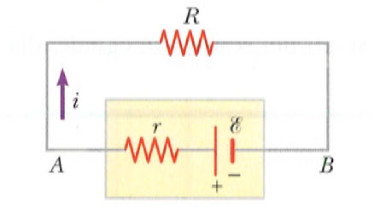
\includegraphics[scale=0.6]{resistenze_circuito.png}
    \centering
    \caption{}
\end{figure}

La (\ref{ddp_res_esterna}) fornisce anche una definizione operativa della f.e.m. di un generatore: essa è uguale alla differenza di potenziale misurata ai capi del generatore a  circuito aperto (\(i = 0\)). 

Poiché l'energia potenziale di una carica positiva \(q\) che percorre il circuito è \(qV\): passando da \(B\) ad \(A\) all'interno del generatore la carica acquista ad opera del campo elettromotore l'energia potenziale \(q\mathcal{E}\) che perde parzialmente dentro il generatore stesso (effetto della resistenza interna) e poi nel resistore (effetto della resistenza esterna) così che in \(B\) la sua energia è nulla. 
Possiamo quindi affermare che la \emph{forza elettromotrice} è numericamente \emph{pari al lavoro fornito dal generatore alla carica unitaria che lo attraversa}. 

Questo bilancio energetico è evidente se moltiplichiamo la (\ref{circuitazione}) per \(dq = i dt\): 
\begin{equation*}
    \mathcal{E} i dt = Ri^2 dt + r i^2 dt
\end{equation*}

Il lavoro fornito dal generatore viene dissipato nelle resistenze del circuito; in termini di \emph{potenza elettrica}
\begin{equation}
    \mathcal{P} = \mathcal{E} i = R i^2 + r i^2 = R_T i^2
\end{equation}


\end{document}